\subsection{Flow Models (Mean)}

We now fit statistical models for the response variable mean TCT. First, we fit a simple linear model, flow.l.one.line.mean. This model only considers log2(Flow) as a predictor.

\vspace{5mm}


\begin{table}[H]
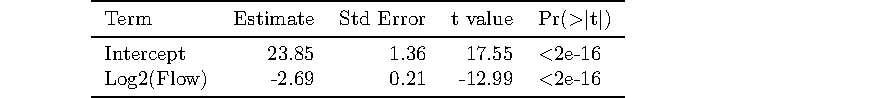
\includegraphics{Chapter4Images/flowlonelinemean.pdf}
\caption{Parameter estimates and standard errors for simple linear model for Mean TCT which only considers log2(Flow) as a predictor. Model: flow.l.one.line.mean. The $R^{2}$ for this model is 0.692.}
\label{fig:meanflow1}
\end{table}

Table~\ref{fig:meanflow1} summarizes flow.l.one.line.mean. The output provides estimates of an intercept of 23.85 and a slope term on log2(Flow) of -2.69. The $ R^{2}$ is 0.692 and the adjusted $R^{2}$ is 0.688.
 

\newpage

We now fit a model, flow.l.tank.mean that also includes the tank number as a factor.  As before, R indicates high significance for the intercept and flow terms.

\vspace{5mm}

\begin{table}[H]
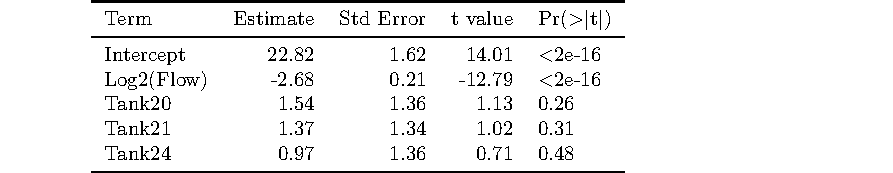
\includegraphics{Chapter4Images/flowltankmean.pdf}
\caption{Parameter estimates and standard errors for a model on Mean TCT that considers tank as a predictor in addition to log2(Flow). Model: flow.l.tank.mean. The $R^{2}$ for this model is 0.699.}
\label{fig:meanflow2}
\end{table}

Table~\ref{fig:meanflow2} summarizes the model flow.l.tank.mean. The estimated intercept for tank 19  is 22.82 and the slope coefficient is -2.68. The $R^{2}$ for the new mean model is 0.699 , however the adjusted $R^{2}$ has now decreased to 0.682. The individual p-values for each tank do not immediately  appear significant. However, this does not guarantee that tank itself is not important. To conclude that, we need to compare this model with a model that does not contain tanks, we can do this using `anova'.
  


\begin{table}[H]
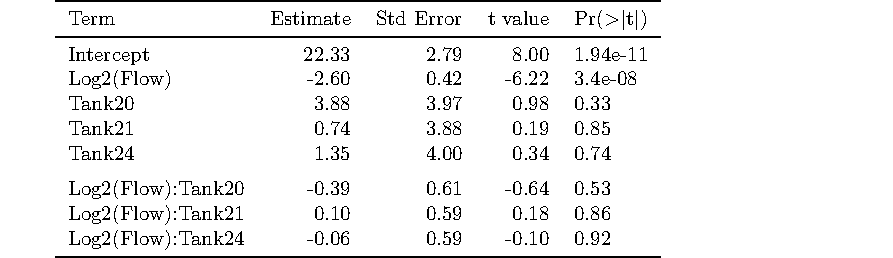
\includegraphics{Chapter4Images/lfourlinemean.pdf}
\caption{Parameter estimates and standard errors for a model on Mean TCT that includes log2(Flow), Tank, and the interaction between log2(Flow) and Tank. Model: flow.l.four.line.mean. The $R^{2}$ for this model is 0.702.}
\label{fig:meanflow3}
\end{table}

 This model includes tank and the interaction between tank and log2(Flow). Hence this allows for both intercepts and slopes to differ between each tank. The results indicate that neither tank, nor the interaction terms are significant. 

\vspace{5mm}


\begin{table}[H]

\includegraphics{Chapter4Images/anovameanF.pdf}
\caption{ANOVA table for flow models.}
\label{fig:anovaflow1}
\end{table}


 Table~\ref{fig:anovaflow1} shows the results of the `anova (extra sum of squares)' test to see which of our models for mean TCT is significant. We first consider the full model  flow.l.four.line.mean that allows for different slopes and different intercepts. Comparing flow.l.four.l.mean with flow.l.tank.mean is a test of equality of slopes. Since the p-value is large, we cannot reject the null hypothesis that the terms are identical. That is, we cannot reject the hypothesis that the slopes do not differ among tanks. Next we compare flow.l.tank.mean with flow.l.one.line.mean, which is a test of differing intercepts. Similarly, we obtain a large p-value (p=0.68) and hence cannot reject the hypothesis that the intercepts do not differ. Thus, as before, we conclude that working with a model that only includes log2(flow) as a predictor is sufficient.
















